\lab{Applications}{PageRank Algorithm}{PageRank Algorithm}
\label{lab:PageRank}
\objective{Explain the basics of the PageRank Algorithm, and some of its applications}

The PageRank algorithm was one of the first algorithms used by Google to classify search results.
It is named after one of the co-founders of Google, Larry Page, and is based on an interesting mathematical model that involves random processes, Markov chains, and eigenvalues.
It ranks pages based upon their connectivity properties with the rest of the internet.
When you run a search on Google's web page, they find every page that contains the keywords you specified and then list them primarily in order of page rank (this isn't true in every case, but it is generally how it works).
As of 2013, PageRank is one of over 200 algorithms used in determining Google's ranking of a website.

The PageRank algorithm works by supposing that a person surfing the internet randomly clicks links on the web pages.
We will notate the probability that the surfer is a particular page $i$ at time $t$ by $PR(i,t)$.
We can write an equation for this probability from one time step to the next using the following notation:
\[PR(i,t+1) = \sum_{j \in M(i)} \frac{PR(j,t)}{L(j)}\]
Where $M(i)$ is the set of pages that link to page $i$, and $L(j)$ represents the number of outbound links on page $j$.
Note that this is simply representing the internet as a Markov chain, just like we discussed in Lab \ref{lab:MarkovGraph}.
We assume that the starting probability is uniform, or in other words that $PR(i,0) = 1/N$.

There are two modifications that still need to be made to this formula.
First, what if a page has no outbound links?
In this case we pretend that the page links to every other page.
It is as if the surfer, upon getting stuck, randomly picks a new page.
Second, we assume that the surfer sometimes gets bored and randomly picks a new page.
The probability that the surfer doesn't get bored is called the damping factor $d$.
A good value is $d=.85$.
Using these modifications we can write our formula as:
\[PR(i,t+1) = \frac{1-d}{N} + d\sum_{j \in M(i)} \frac{PR(j,t)}{L(j)}\]
Note that $N$ is the total number of web pages.
We then say that the page rank of a particular web page is the value
\[PR(i) = \lim_{t\to \infty} PR(i,t)\]

Mathematically, the page rank is the steady state probability of our modified Markov chain.
We can rewrite this as a matrix equation:
\[R(t+1) = d K R(t) + \frac{1-d}{N} \begin{pmatrix}1\\\vdots\end{pmatrix}\]
Where $R_i(t) = PR(i,t)$.
The matrix $K$ is defined by:
\[K_{ij} = \begin{cases} \frac{1}{L(j)} & \mbox{ if j is linked to i} \\
	0 & \mbox{ otherwise} \end{cases}\]

We can write $K$ neatly as follows:
\[K = (B^{-1}A)^T\]

Where $A$ is the adjacency matrix for the directed graph (the edges are links) and $B$ is the diagonal matrix containing the number of links leaving each vertex.
Remember that we have to modify our graph so that any page without outbound links points to every other page.
Otherwise these definitions don't make sense (for example $B^{-1}$ will not be well-defined).
In practice, you should \textit{never} construct a diagonal matrix, invert it, then do matrix multiplication.
That would be a series of very computationally expensive and unnecessary operations.
Store the diagonal entries of $B$, compute the inverse by taking their reciprocal, then perform the matrix multiplication by multiplying each of the rows of $A$ by each of the corresponding  entries of the diagonal of $B^{-1}$.
These operations are mathematically equivalent versions of the inversion and multiplication, but they are much more efficient.

A useful way to think of this algorithm is to think in terms of voting.
Every link that I place on my web page is a vote for the web page that it points to.
Additionally, if I am more prestigious then my votes count for more.

\begin{problem}
Included with this lab is a sample data set.
There is a comment at the top.
Each of the remaining lines represents a link going from one web page to another.
Each line consists of two integers.
The first is the index of the web page containing the link.
The second is the index of the web page pointed to by the link.
Write a function that constructs the adjacency matrix by reading in the data from file.
Store the data in a \li{scipy.sparse.dok_matrix}.

Recall that you can open a file (in read mode) using an \li{with} construct
\begin{lstlisting}
with open(filename, 'r') as f:
    # do stuff here.
\end{lstlisting}
Once you have opened the file you can iterate through the lines of the file by doing something like
\begin{lstlisting}
for L in f:
    # 'L' iterates through each line of 'f'
    # You can do stuff with the lines here.
\end{lstlisting}
For each line, you will want to split the line into its space-separated parts.
This can be done with something like \li{l.strip().split()}.
The \li{strip()} method removes endline characters and the \li{split()} method splits the string into the space-separated parts.
Once you have read in the line, you can use a try-except block to avoid issues with errors that occur with the strings you obtain 
\end{problem}

There are several ways to solve for $\lim_{t \to \infty} R(t)$.
One option is simply iterate the equation for $R(t)$ until $\norm{R(t)-R(t-1)}$ is sufficiently small.

\begin{problem}
\label{prob:pagerank_dense_iter}
Write an implementation of the page rank algorithm that computes the steady state $R$ iteratively, as described above.
Your function should accept a file name for the data, a floating point value for $d$, and a size \li{n} that defaults to \li{None}.
When the size is not None, your function should only consider the upper left $n \times n$ portion of the array.
\end{problem}

Another method for computation assumes a steady state $R$ and solves the resulting system:
\[(I-dK)R = \frac{1-d}{N} \begin{pmatrix}1\\\vdots\end{pmatrix}\]
We won't have you implement this version of the algorithm here.

Another way to solve this problem is to make it into an eigenvalue problem.
Since $R$ can be viewed as a vector of probabilities we can rewrite $\left(\begin{smallmatrix}1\\\vdots\end{smallmatrix}\right) = E R$, where $E$ is a matrix of all ones.
Thus the equation becomes:
\[R = (dK + \frac{1-d}{N}E)R\]
Since $(dK + \frac{1-d}{N}E)$ will be a strictly positive stochastic matrix (each column sums to one) the Perron-Frobenius theorem guarantees that this eigenvalue equation corresponds to the largest magnitude eigenvalue and that the eigenvector is unique.
This means that, by finding the eigenvector corresponding to the largest eigenvalue of $(dK + \frac{1-d}{N}E)$, we can find $R$.
The first option for finding $R$ (the iterative approach) is equivalent to using a numerical method called power iteration to find the eigenvalues of this system.
As we have formulated the eigenvalue problem here, it cannot be stored easily in one of SciPy's sparse matrix types, but it is still possible to work with eigenvalue solvers that exploit the symmetries of this matrix.

\begin{problem}
Write another version of the algorithm that uses the eigenvalue solver in \li{scipy.linalg} to compute the page rank within a group of web pages.
You will want to solve the eigenvalue problem above, then return the eigenvector corresponding to the eigenvalue of largest magnitude.
It should accept the same inputs as your solution to Problem \ref{prob:pagerank_dense_iter}.
\end{problem}

The computed value for $R$ gives the page rank associated with each web page.

This algorithm has been used in several settings (primarily in academia).
For example, it has been used to rank graduate institutions, to rank impact factor of journals and has even been used in some biological applications.

Let's try implementing the Page Rank algorithm on a small subset of the internet.
The SNAP graph library includes a variety of medium sized data sets that can be used for analysis.
Their data sets can be found at \url{http://snap.stanford.edu/data/index.html}.
Download one of the data sets there so you can use it to test your page ranking algorithm.

The \li{matplotlib.pyplot.spy} command of this adjacency matrix yields the plot shown in figure \ref{fig:WebSparse}

\begin{figure}
\centering
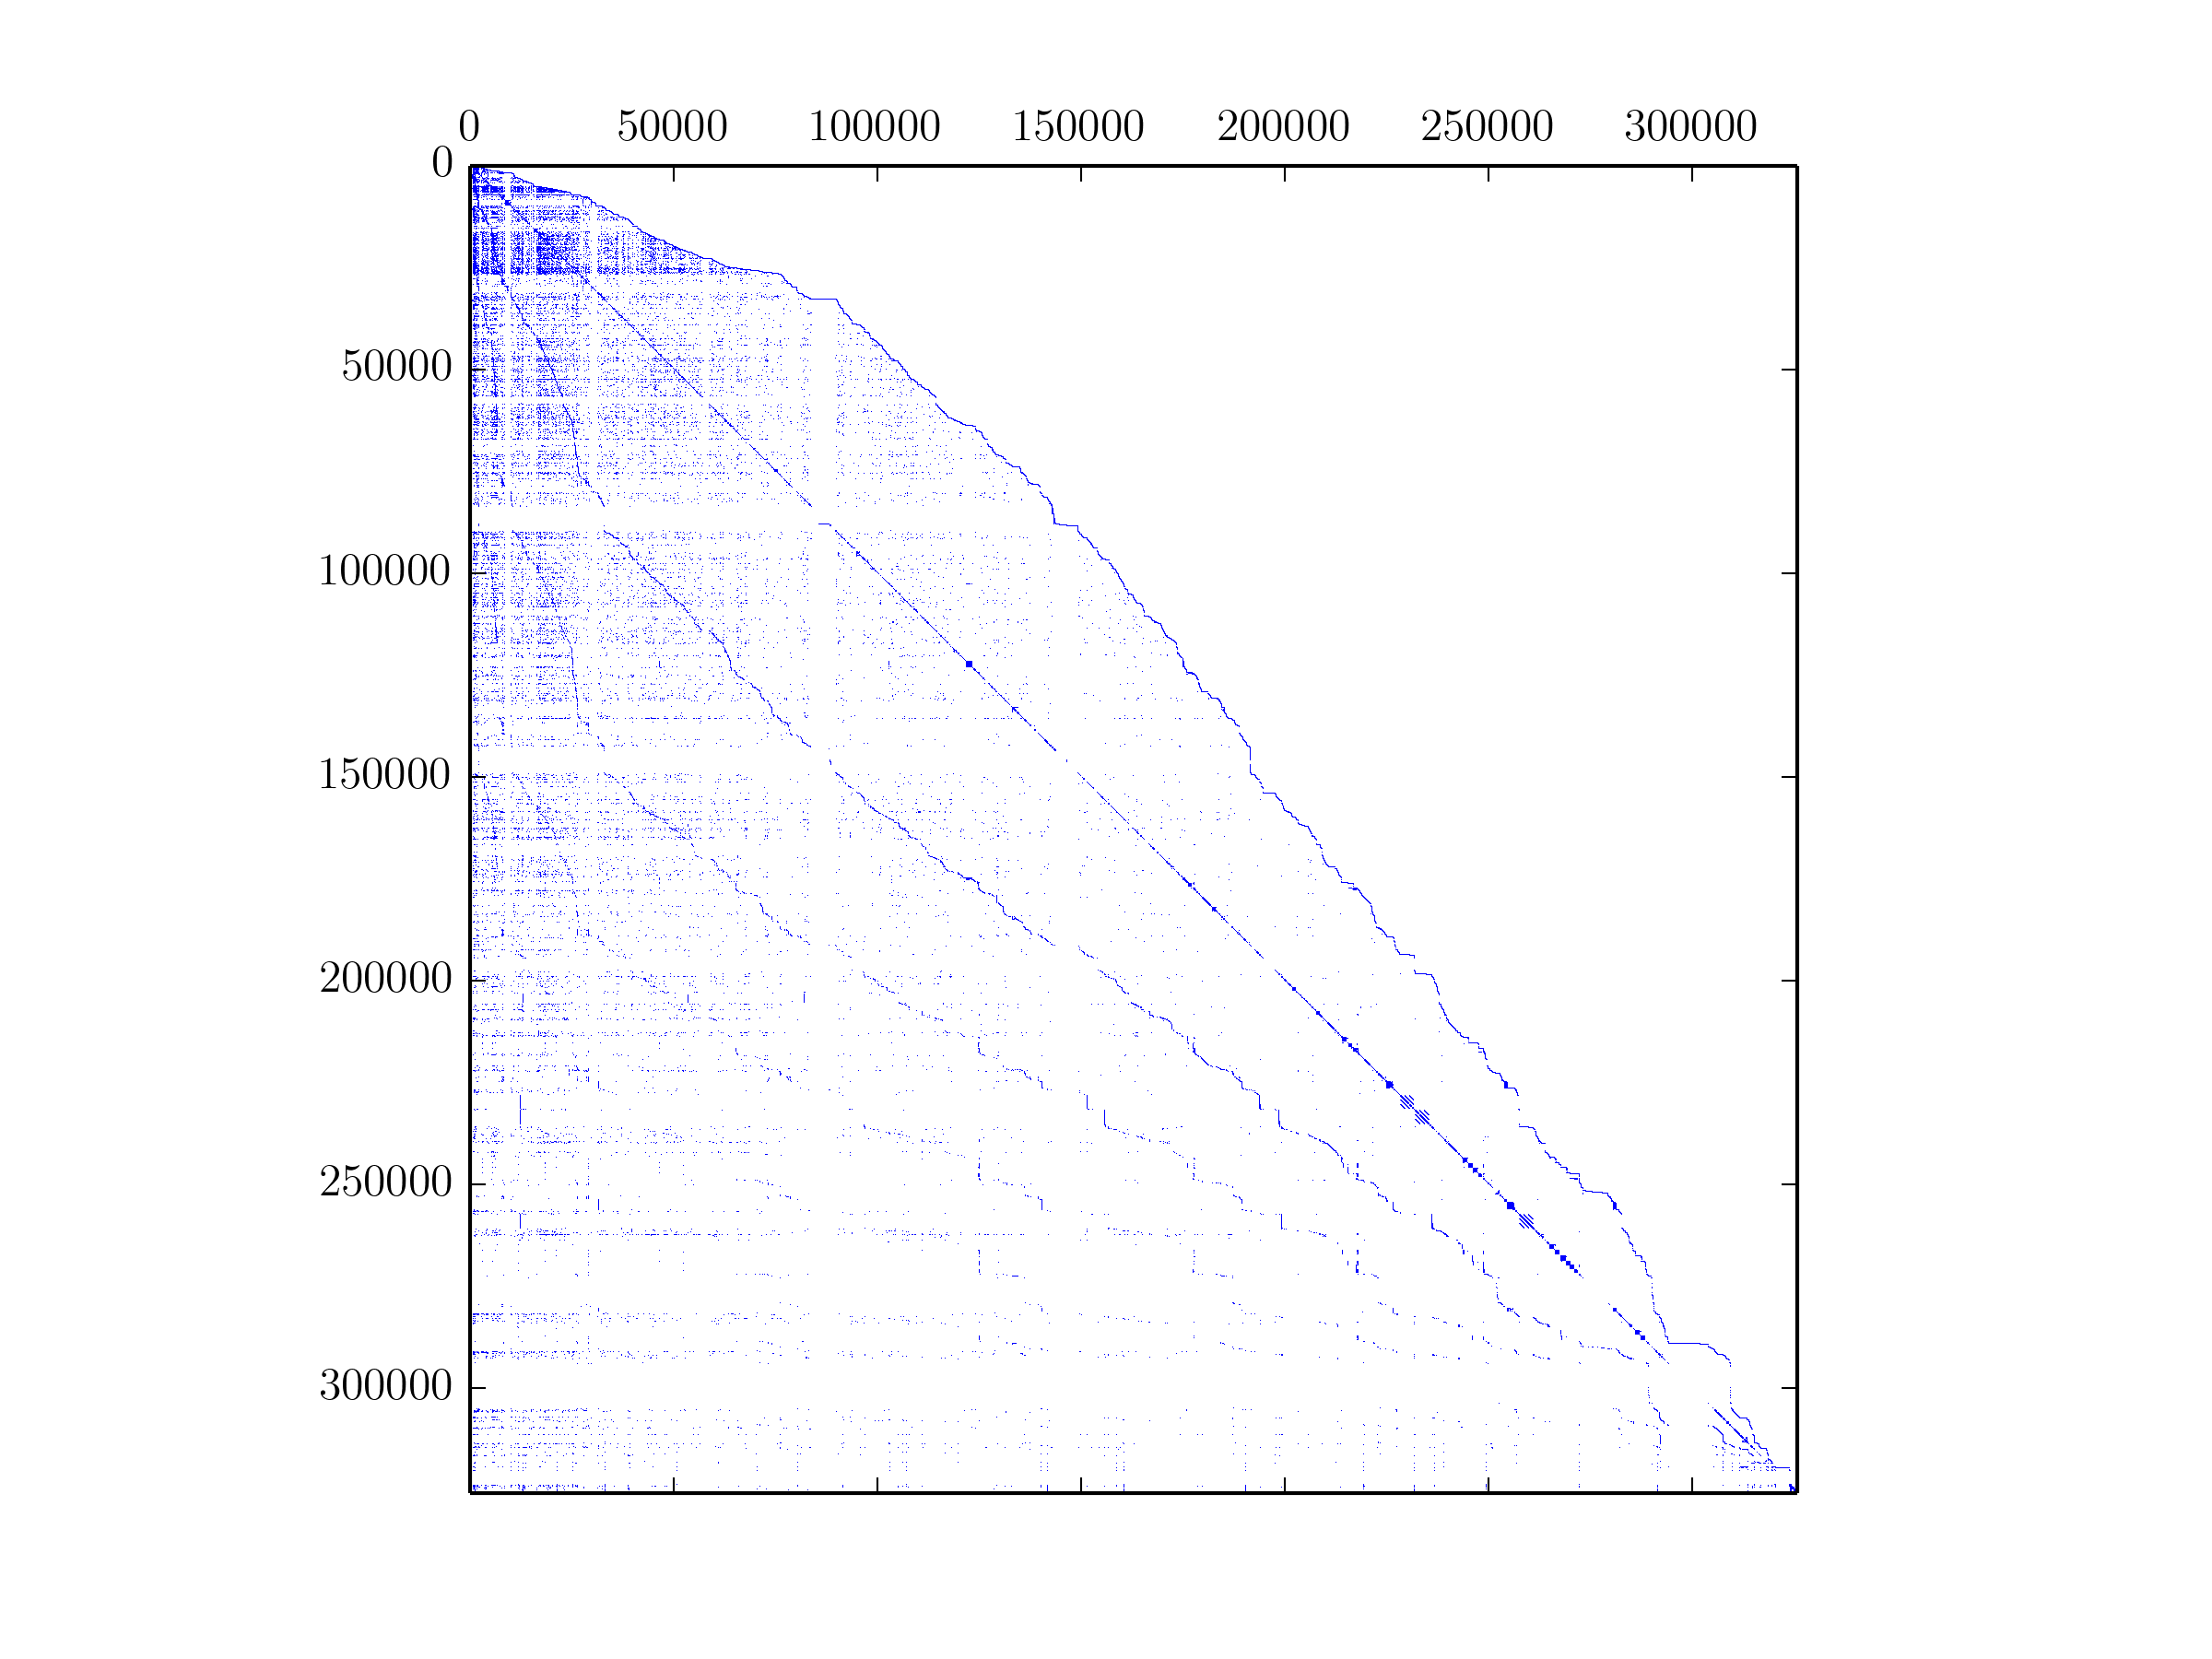
\includegraphics[width=\textwidth]{sparse_web.png}
\caption{\li{spy} command on the adjacency matrix corresponding to the websites supported by Notre Dame University in 1999.
Data was taken from the SNAP datasets.}
\label{fig:WebSparse}
\end{figure}

\begin{problem}
Use your previous implementations of the Page Rank algorithm to calculate the Page Rank of the first 3500 web pages in the data set you have downloaded.
Which page has the highest page rank, and what is the value of the page rank?
\label{prob:pg_calc}
\end{problem}

\begin{problem}
The iterative method allows for an easy implementation using sparse matrices.
Write an implementation of the iterative Page Rank algorithm that uses sparse matrices.
Use it to compute the Page Ranks for all the pages in the data set.
Which page has the highest rank?

Hint: You will want to convert your sparse matrix to a \li{csc_matrix} or a \li{csr_matrix} to perform the computations.
\end{problem}
